70. $\cfrac{(x^2+3x-10)(x^2+3x+5)}{3x^2-7x+2}\geqslant0\Leftrightarrow\cfrac{(x+5)(x-2)((x+1,5)^2+2,75)}{(x-2)(3x-1)}\geqslant0.$ Применив метод интервалов, найдём ответ: $x\in(-\infty;-5]\cup\left(\cfrac{1}{3};2\right)\cup(2;+\infty).$
\begin{figure}[ht!]
\center{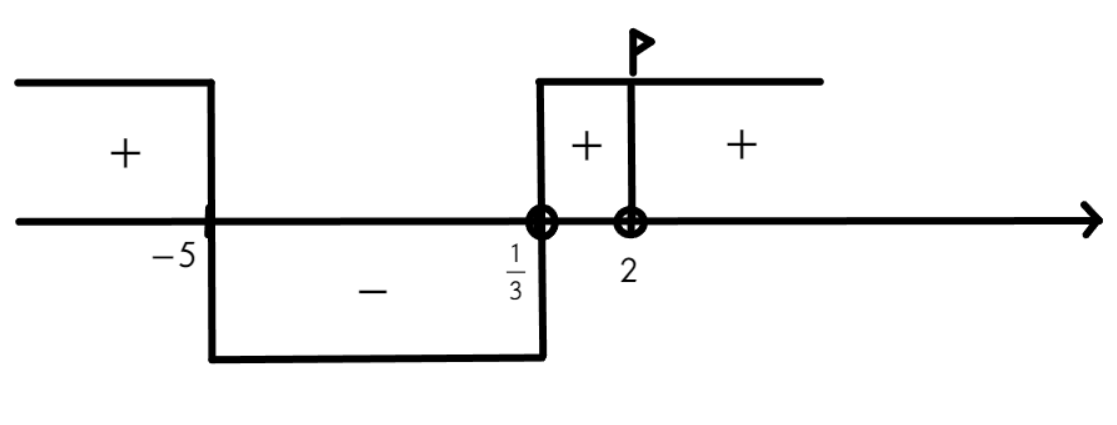
\includegraphics[scale=0.35]{ner9-70.png}}
\end{figure}\\
